\subsection{Metodi sperimentali per la valutazione dell'esplorazione} \label{subsec:experimental_expl_eval}
In questa sotto-sezione si riportano i vari metodi sviluppati durante le fasi di test, ma che sono stati rimpiazzati da una versione successiva più accurata, fino ad arrivare a quello utilizzato negli esperimenti, ed esposto in \ref{subsec:expl_eval_frontier_NCC}.

\subsubsection{Simple Exploration}
Questo metodo è stato utilizzato nelle fasi iniziali per verificare la variazione di probabilità delle celle in tempi di simulazione ragionevoli. 
Esso non tiene conto del SINR per valutare la copertura di un cella, ma controlla soltanto che il suo centro sia abbastanza vicino ad un sensore.
Per ovvi motivi, tale metodo è stato rapidamente sostituito dai successivi.

\subsubsection{Local Square Interference Exploration (LSIE)}
In questa variante, si va a valutare la copertura di una cella tramite il livello di SINR calcolato nel suo centro, rendendo il requisito di copertura della cella simile a quello della copertura utente.
La novità principale è quella di non considerare tutte le celle della matrice, ma soltanto quelle che rientrano all'interno di un'area quadrata centrata nella posizione dell'agente, di lato \texttt{2$\cdot$EXPLORATION\_RADIUS} (Figura \ref{fig:esempio_LSIE}).
\begin{SCfigure}[1][h]
    \centering
    \caption[Esempio dell'area valutata con il metodo LSIE]{Esempio dell'area considerata dal metodo LSIE; si osserva come le celle presenti negli angoli dell'area siano difficilmente raggiungibili dal segnale dell'agente.}
    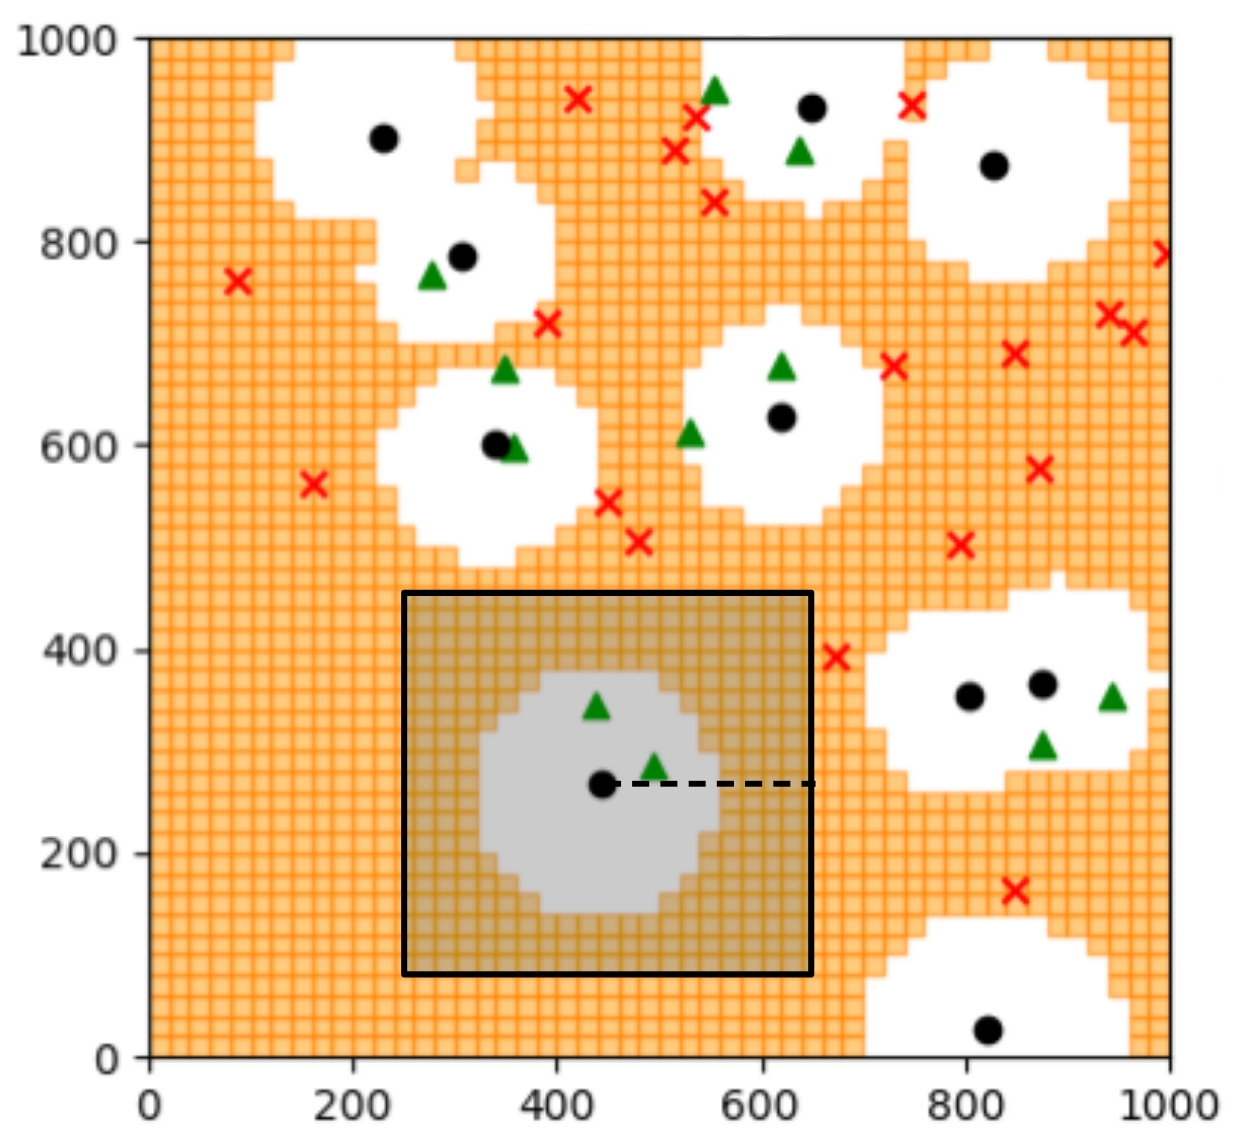
\includegraphics[width=0.5\textwidth]{img/ch3/esempio_LSIE.jpg}
    \label{fig:esempio_LSIE}
\end{SCfigure}

Inoltre si vanno a considerare soltanto le interferenze provenienti da sensori relativamente vicini all'agente, in quanto una eccessiva distanza rende il segnale d'interferenza trascurabile; questa considerazione permette di avere un minor numero di agenti nel calcolo del SINR, alleggerendo il costo computazionale.
Si osserva come la scelta del valore di \texttt{EXPLORATION\_RADIUS} sia critica, in quanto  un raggio maggiore implica una visione più approfondita dell'ambiente da parte dell'agente, comportando però una minore velocità del metodo.
\textbf{Sperimentalmente} si è osservato che ponendo \texttt{EXPLORATION\_RADIUS=200} si ha un'esplorazione completa dell'area intorno ad un punto, mantenendo un buon tempo di simulazione.
Il problema di questa variante è che, data la forma quadrata dell'area, si andranno a considerare anche le celle negli angoli, che molto probabilmente non saranno mai coperte dal segnale dell'agente (Figura \ref{fig:esempio_LSIE}).


\subsubsection{Local Circle Interference Exploration (LCIE)}
Rispetto al metodo precedente questa variante modifica la forma dell'area osservata, passando dall'utilizzo di un'area quadrata ad una circolare, rimuovendo quindi le celle che prima si trovavano negli angoli; questo porta ad un'ulteriore aumento di velocità del processo di valutazione, essendosi ridotto il numero di celle da osservare.
\begin{figure}[h]
    \centering
    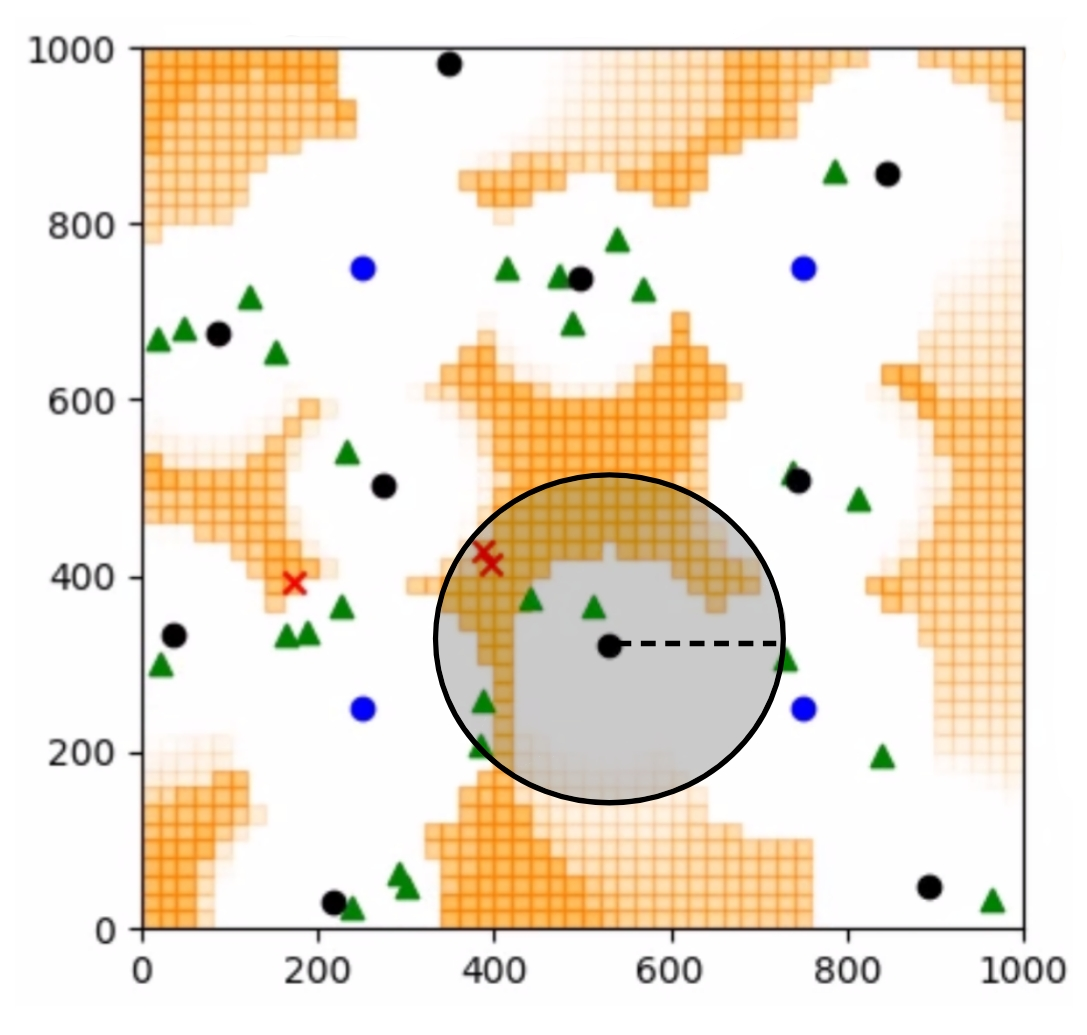
\includegraphics[width=0.5\textwidth]{img/ch3/esempio_LCIE.jpg}
    \caption[Esempio dell'area valutata con il metodo LCIE]{Esempio di area considerata dal metodo LCIE.}
    \label{fig:esempio_LCIE}
\end{figure}

\subsubsection{Local Square Interference Exploration, Neighbour Cell Control (LSIENCC)}
Implementata prima della \textit{Local Circle Interference Exploration}, questo metodo aggiunge una predizione sul livello di copertura di alcune celle quando sono soddisfatte alcune condizioni.
Tale predizione si basa sull'osservazione che, se il SINR calcolato in una cella è abbastanza alto, allora con molta probabilità anche quello delle celle adiacenti supererà la soglia richiesta.
Seguendo tale euristica, è possibile ridurre drasticamente i tempi di valutazione dell'esplorazione di quegli agenti isolati rispetto al resto della rete: infatti, la distanza da gli altri agenti fa sì che il livello di SINR rimanga abbastanza uniforme lungo l'area.